% ============================================================================
%  Chapter 1 -- Introduction
% ----------------------------------------------------------------------------
%  FORMAT CONVERSION of the six approved section drafts under
%  thesis_writing/chapter_1/section_1_1_v1.md .. section_1_6_v1.md, after
%  their full scientific/coherence/claim audit
%  (thesis_writing/chapter_1/chapter_1_full_audit_v1.md). Scientific prose is
%  preserved verbatim from the audited v1 drafts; only changes required for
%  valid LaTeX have been made (markdown heading/bold syntax, em-dashes,
%  citation commands, cross-references) -- see the itemised list below. The
%  audit's own MAJOR/MINOR/STYLE prose-revision recommendations are NOT
%  applied here; this pass is integration/formatting only.
%
%  Source-file mapping (kept unchanged as source/history, not further edited):
%    1.1 Background and Motivation  <- chapter_1/section_1_1_v1.md
%    1.2 Problem Statement          <- chapter_1/section_1_2_v1.md
%    1.3 Research Gap               <- chapter_1/section_1_3_v1.md
%    1.4 Research Questions         <- chapter_1/section_1_4_v1.md
%    1.5 Contributions              <- chapter_1/section_1_5_v1.md
%    1.6 Thesis Organization        <- chapter_1/section_1_6_v1.md
%
%  MECHANICAL CHANGES APPLIED (conversion only, no content change):
%    - Markdown "# 1.N Title" headings -> \section{Title} with a
%      \label{sec:ch1-...} slug, following Chapter 3's ch3-prefixed
%      labelling convention (Chapter 2 does not prefix; Chapter 1's section
%      names are generic enough -- "motivation", "contributions" -- that the
%      prefixed form was chosen to avoid any future collision).
%    - Markdown "**text**" -> \textbf{text} (RQ/contribution lead-ins),
%      matching the bold-lead-phrase convention already used in Chapter 2's
%      positioning section (e.g. "\textbf{The two adaptation strategies
%      (RQ1).}", chapter_2.tex around line 1002) and in Chapter 3's
%      \textbf{Procedure (...).} lead-ins.
%    - The four numbered contributions -> \begin{enumerate}...\end{enumerate}
%      with a \textbf{...} lead per \item -- \texttt{enumerate} is precedented
%      in this thesis (Chapter 3's two step-by-step procedures,
%      chapter_3.tex:974/1005); \texttt{itemize} is not used anywhere and was
%      not introduced here either.
%    - Literal "Section 1.N" / "Chapter N" cross-references -> \ref{} against
%      this chapter's own new sec:ch1-* labels and the existing ch:* chapter
%      labels defined by the DEI template, matching how Chapters 2/3
%      universally cross-reference (never a bare number). Section 1.6's
%      five paragraphs keep each chapter's descriptive title in prose
%      (\emph{...}) alongside \ref{} for the number -- content preserved,
%      only the number itself is now dynamic rather than hardcoded.
%    - Two Unicode em-dash-set-off clauses (1.3's and 1.4's closing/opening
%      sentences) -> LaTeX "---", unspaced, matching this thesis's dominant
%      em-dash convention (e.g. chapter_2.tex "baseline---the
%      independent-adapter-averaging case").
%    - "retention-plasticity" (hyphen, 6 occurrences across 1.1-1.3) ->
%      "retention--plasticity" (en-dash), matching Chapter 2's own rendering
%      of the identical term (chapter_2.tex:508, "retention--plasticity
%      comparison that motivates the primary research question") and the
%      cognate "stability--plasticity" (chapter_2.tex:87-88). This is the
%      one content-adjacent fix applied, and it is purely typographic
%      (identified as MINOR Issue 3 in the full-chapter audit and explicitly
%      named as a required special-character conversion for this pass); no
%      wording, claim, RQ, or contribution was altered.
%    - No other MAJOR/MINOR/STYLE item from chapter_1_full_audit_v1.md was
%      applied in THIS integration pass (Issues 1, 2, 4, 5, 6, 7 were left
%      open, deliberately, pending a separate scientific-revision pass).
%
%  MINIMAL REVISION PASS (2026-09-14, chapter_1_revision_report_v2.md):
%    applied the audit's MAJOR issue (1) and four of its five MINOR issues
%    (2, 4, 5, 6) to both this file and the corresponding v1 markdown
%    sources, keeping them synchronised; Issue 3 (retention--plasticity
%    dash) was already applied during the original integration pass above
%    and is unchanged here; Issue 7 (STYLE, Section 1.6 paragraph rhythm)
%    was reviewed and deliberately skipped as subjective -- see the
%    revision report for the full per-issue reasoning. No RQ, no
%    contribution's C-to-RQ mapping, no citation, and no chapter/section
%    structure was changed by this pass.
%
%  CITATION SYSTEM: biblatex, style=numeric-comp, backend=biber, configured
%    in DEIthesis.cls (line ~74). This is the ACTUAL configured style, not
%    the "style=authoryear" comment carried in Chapter 2/3's own headers
%    (a known-stale comment there, left untouched per instruction not to
%    modify Chapters 2/3 in this pass -- see
%    thesis_agent/reports/chapter_1_preparation_audit.md Section 20).
%    \parencite{key} and \textcite{key} are style-agnostic biblatex commands
%    and render as numeric, e.g. "[6]", under numeric-comp; they are used
%    directly here (not as temporary author-year placeholders) because every
%    key Chapter 1 cites was already confirmed to exist in references.bib
%    before drafting (thesis_agent/reports/chapter_1_preparation_audit.md
%    Section 13/17).
%
%  FORWARD REFERENCES: none left unresolved. Every "Chapter N" mention
%    resolves to the existing chapter labels defined elsewhere in this
%    project (ch:literature, ch:methodology, ch:experimental-setup,
%    ch:results, ch:discussion-conclusion); every "Section 1.N" mention
%    resolves to one of this chapter's own six new sec:ch1-* labels.
%
%  SUPERVISOR-FACING PRECISION REVISION (2026-09-23): scientific wording of
%    1.1-1.6 revised for consistency with the implemented experiments --
%    CIL framed as a subtype of continual learning; SimpleAvg defined as
%    independent per-step rank-80 adapters whose reconstructed dense updates
%    are arithmetically averaged once after the sequence; RankExt defined as
%    one persistent adapter with hard-frozen, still-active earlier rank
%    blocks; stabilisation (RQ2) made RankExt-focused; open/restricted
%    evaluation framed as primary measure + complementary diagnostic.
%    RQ4 and the protocol-depth contribution were REMOVED (three research-gap
%    components, three RQs, three contributions now). Figures 1.1 and 1.2
%    added from thesis_writing/pictures (baked-in captions cropped off; copies
%    under figures/chapter1/). The "four numbered contributions" note above
%    is historical.
% ============================================================================

\chapter{Introduction}
\label{ch:introduction}

\section{Background and Motivation}
\label{sec:ch1-motivation}

Large vision-language models pretrained on broad, weakly supervised
image-text corpora have reshaped how visual recognition systems are built.
Vision encoders trained under this paradigm, such as CLIP's, learn image
representations that transfer well across a wide range of downstream
recognition tasks without task-specific pretraining
\parencite{radford2021learning}. Such backbones offer an attractive starting
point for building a recognition system: rather than training a new model
per task from randomly initialised weights, a single strong,
general-purpose representation can instead be adapted to the task at hand.

Adapting a model of this scale separately for every downstream task is,
however, costly. Fully fine-tuning the entire backbone for each new task
requires storing a full copy of its parameters per task and repeating
expensive optimisation over the whole parameter set, a cost that scales
with the number of tasks supported. Parameter-efficient fine-tuning
addresses this problem directly: rather than updating all of a pretrained
model's weights, only a small number of additional parameters are
introduced and trained, while the backbone itself remains frozen. Low-rank
adaptation (LoRA) is a widely used instance of this idea, in which a
trainable low-rank update is added alongside a frozen weight matrix, so
that adaptation is expressed through a small number of additional
parameters rather than by modifying the backbone itself
\parencite{hu2021lora}. This substantially reduces the storage and compute
associated with adapting such a model to a new task, while retaining the
representational strength of the frozen backbone.

This picture implicitly assumes that the data required for a downstream
adaptation is available together, so that a single adaptation can be
trained and then deployed. The assumption becomes more restrictive in
continual learning, and more specifically in class-incremental learning,
where new classes arrive sequentially in disjoint groups. In the
rehearsal-free setting considered in this thesis, only the current step's
training data is available: examples from earlier steps are not retained
for replay, while classes belonging to later steps have not yet been
observed. Figure~\ref{fig:ch1-cil-setting} illustrates this setting.

\begin{figure}[htbp]
\centering
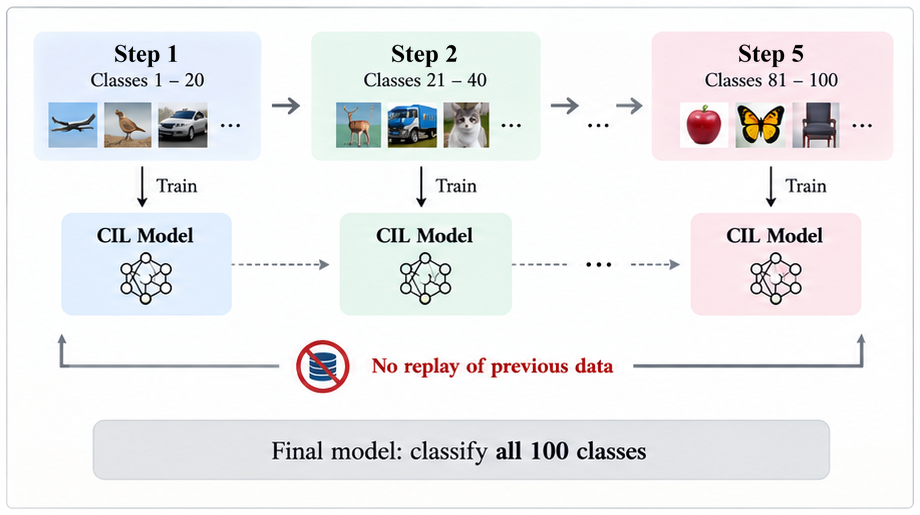
\includegraphics[width=0.85\textwidth]{figures/chapter1/ch1_rehearsal_free_cil_setting.png}
\caption[Rehearsal-free class-incremental learning setting]{Rehearsal-free
class-incremental learning setting used in this thesis. Disjoint groups of
classes arrive sequentially, no examples from earlier steps are replayed,
and the final model must classify all classes encountered across the
sequence. Conceptual redrawing based on the class-incremental learning
setting of \textcite{masana2020classincremental}.}
\label{fig:ch1-cil-setting}
\end{figure}

Training in this sequential manner exposes a central difficulty of
continual learning, catastrophic forgetting
\parencite{kirkpatrick2017overcoming}. In conventional sequential training,
updating parameters on newly arriving classes can degrade representations
or decision boundaries that support classes learned earlier. A continual
learner must therefore balance two competing requirements: it must remain
plastic enough to genuinely acquire new classes, while remaining stable
enough to retain competence on classes already learned. This tension,
commonly referred to as the retention--plasticity trade-off, is a central
challenge in class-incremental learning \parencite{delange2022continual}.

This difficulty is compounded under a rehearsal-free constraint, in which
no examples from earlier steps are stored and replayed alongside new data.
Rehearsal-based approaches can partially counteract forgetting by
re-exposing the model to past examples, but doing so requires retaining
raw data, which may be undesirable or infeasible for reasons of storage,
privacy, or deployment. Under a rehearsal-free constraint, information from
earlier steps must be preserved through retained model state rather than
through replay of the original training examples. This removes a direct
source of supervision for earlier classes and makes retention more
challenging.

Placing parameter-efficient adaptation in this sequential, rehearsal-free
setting raises a further, more specific design question. If each
incremental step produces its own low-rank adaptation, or extends a
shared one, how should the adaptations associated with different steps be
maintained, combined, or allowed to interact as training proceeds? Because
independently learned low-rank updates may interact when combined, the
integration rule itself can also influence continual-learning performance.
This thesis considers two structurally different answers. The first,
referred to here as SimpleAvg, trains an independent low-rank adapter at
each step, reconstructs the dense update induced by each adapter, and
combines these dense updates once, after the full incremental sequence, by
arithmetic averaging. The second, referred to here as RankExt, instead
maintains one persistent adaptation whose rank capacity is extended at each
step: new rank capacity is appended for the incoming classes, while
previously learned rank blocks remain active and are hard-frozen, so that
only the newly appended capacity is trained. Within this comparison,
SimpleAvg provides a reference based on independently trained per-step
adaptations, while RankExt tests how closely a single persistent model
whose adaptation capacity is introduced incrementally can approach that
reference. Combining independently trained components after the fact, and
extending a single adaptation's capacity over time, both build on broader
ideas in the literature reviewed in Chapter~\ref{ch:literature}; this
thesis examines the retention--plasticity behaviour each produces under one
shared rehearsal-free protocol. Figure~\ref{fig:ch1-integration-strategies}
summarises the two strategies.

\begin{figure}[htbp]
\centering
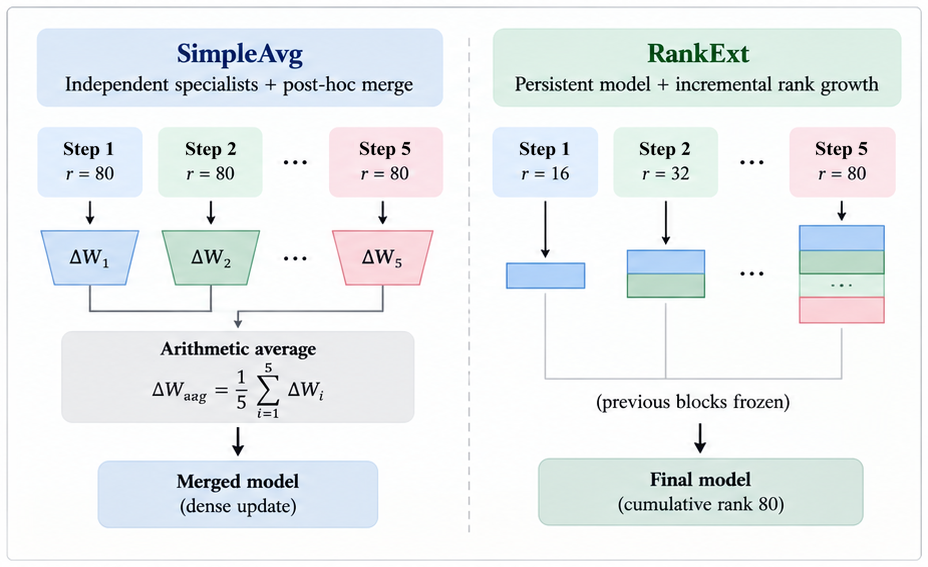
\includegraphics[width=0.9\textwidth]{figures/chapter1/ch1_simpleavg_vs_rankext.png}
\caption[The two LoRA integration strategies compared]{Overview of the two
LoRA integration strategies compared in this thesis. SimpleAvg trains
independent per-step adapters and combines their reconstructed dense
updates once after the sequence, whereas RankExt maintains a persistent
adapter whose capacity grows incrementally while previously learned blocks
remain frozen and active. The ranks shown correspond to the primary
$5\times20$ configuration. Original schematic.}
\label{fig:ch1-integration-strategies}
\end{figure}

Performance under either integration strategy can still be affected by
interference, although that interference arises differently in the two
families: independently learned updates may conflict when they are merged
in SimpleAvg, whereas newly introduced capacity in RankExt must coexist
with the frozen contributions retained from earlier steps. Additional
mechanisms are commonly introduced to limit such interference. Knowledge
distillation, in which a model is encouraged to match the outputs of an
earlier version of itself, and orthogonality-based regularisation, which
discourages a new update from overlapping with directions already used by
previous updates, are two such mechanisms examined in this thesis. Both are
established continual-learning tools; this thesis examines them primarily
within the persistent RankExt family, asking what role each plays there,
alone and in combination.
Section~\ref{sec:ch1-problem-statement} turns these observations into a
precise statement of the problem this thesis addresses.

\section{Problem Statement}
\label{sec:ch1-problem-statement}

The problem this thesis addresses can now be stated more precisely. A
pretrained visual backbone is adapted, using a parameter-efficient
mechanism, to a sequence of incremental steps, each introducing a disjoint
group of classes the model has not previously encountered. No training
examples from earlier steps are retained for replay: at each step, only
the classes introduced at that step are available for training. After
each incremental step, a class-incremental learner is expected to classify
over the cumulative set of classes encountered so far, rather than only the
classes introduced most recently. Under these constraints, the system must extend its competence to the new
classes of the current step while preserving its competence on classes
introduced at earlier steps, and it must do so without abandoning the
parameter-efficiency that motivated adopting a low-rank adaptation
mechanism in the first place. This is the retention--plasticity trade-off
introduced in Section~\ref{sec:ch1-motivation}, now situated concretely
within a rehearsal-free, parameter-efficient, class-incremental setting.

Because adaptation here is expressed through low-rank updates rather than
through full fine-tuning, a further, architecture-level problem arises.
Section~\ref{sec:ch1-motivation} raised this informally; formally, across
successive incremental steps, how should the resulting low-rank
adaptations be retained, combined, or extended? This thesis studies two
contrasting answers, treated as its two experimental families. Under the
first, SimpleAvg, an independent low-rank adapter is trained at each step;
the dense updates induced by these independently trained adapters are
reconstructed and combined once, after the full incremental sequence, by
arithmetic averaging. Under the second, RankExt, a single persistent
low-rank adaptation is maintained throughout, and its cumulative rank grows
over the sequence: previously learned rank blocks are retained and
hard-frozen while new rank capacity is appended at each step. Within this
comparison, SimpleAvg provides a reference based on independently trained
per-step adaptations, while RankExt tests how closely a single persistent
model whose adaptation capacity is introduced incrementally can approach
that reference. The precise mechanics of both families are given in
Chapter~\ref{ch:methodology}.

A further part of the problem is whether additional stabilisation can
improve the persistent RankExt family, where newly introduced capacity must
coexist with frozen earlier blocks. Two stabilisation mechanisms are
considered for this purpose: knowledge distillation, which encourages a
model to remain consistent with an earlier version of itself, and FactorOrth
regularization, an orthogonality-based penalty whose concrete formulation
is family-specific and which discourages a new update from occupying
directions already used by previous updates. This
thesis therefore examines knowledge distillation and FactorOrth
regularization within RankExt, while the corresponding SimpleAvg variants
are retained as supporting comparative evidence. Whether either mechanism,
or their combination, benefits RankExt is treated here as an open empirical
question rather than a settled one.

Finally, how retention is measured is itself part of the problem. A
class-incremental system's reported performance can differ substantially
depending on whether predictions are made freely over every class
encountered so far, or restricted to the classes belonging to one
already-identified incremental step \parencite{delange2022continual}.
This thesis therefore reports task-agnostic open evaluation as the primary
class-incremental measure and uses task-oracle restricted evaluation as a
complementary diagnostic of within-group discrimination and cross-group
competition.

Taken together, this thesis seeks to understand how the architecture used
to integrate successive low-rank adaptations, the stabilisation mechanisms
applied within the persistent RankExt family, and the conditions under
which retention is evaluated, jointly shape the retention--plasticity trade-off in
rehearsal-free class-incremental learning. Establishing where the existing
literature leaves this question open is the task of
Section~\ref{sec:ch1-research-gap}.

\section{Research Gap}
\label{sec:ch1-research-gap}

Section~\ref{sec:ch1-problem-statement} situated this problem in terms of
integrating successive low-rank adaptations, stabilising them against
interference, and evaluating the retention this produces, all within a
rehearsal-free class-incremental setting. The individual components
considered in this thesis build on established lines of work in
parameter-efficient fine-tuning, continual learning, knowledge
distillation, orthogonality-based regularisation, and model merging. What
is less directly characterised in the literature reviewed in
Chapter~\ref{ch:literature} is how these components interact when examined
within one shared, controlled rehearsal-free class-incremental framework.
In particular, this thesis focuses on the behaviour of a persistent
rank-extension strategy whose capacity grows incrementally while previously
learned rank blocks remain frozen and active, and uses independent per-step
adaptation with post-hoc averaging as a reference point against which that
behaviour can be interpreted.

The first component of this gap concerns integration architecture.
Persistent or growing low-rank adaptation has precedent in recent
continual-LoRA methods \parencite{wu2025sdlora,he2025cllora}, while the
combination of independently trained adaptations through weight averaging
is established in the model-merging literature
\parencite{wortsman2022model}. The literature reviewed in
Chapter~\ref{ch:literature} does not provide a directly matched comparison
between these two integration philosophies under the same rehearsal-free
class-incremental pipeline, with the same backbone, class partition, and
evaluation protocol. The closest methods reviewed in
Chapter~\ref{ch:literature} differ in architecture, training procedure,
evaluation protocol, or deployment assumptions, preventing a direct
like-for-like comparison of the two strategies considered here. This
comparison is especially informative for RankExt, since it asks how
closely a single persistent model whose adaptation capacity is introduced
incrementally can approach the reference provided by independently trained
per-step adaptations and post-hoc averaging.

The second component concerns stabilisation within the persistent RankExt
family. RankExt protects previously learned rank blocks structurally by
freezing them, but newly introduced capacity must still coexist with and
complement those frozen contributions. Knowledge distillation and
orthogonality-based regularisation are established continual-learning
mechanisms \parencite{li2016learning,wang2023orthogonal}: distillation
encourages the current model to remain consistent with the outputs of an
earlier model state, while orthogonality-based regularisation discourages
new low-rank updates from occupying directions already used by earlier
ones. Their contribution in this specific persistent growing-rank setting,
and particularly their interaction when combined, is not established by
the prior work reviewed here. The corresponding SimpleAvg variants are
retained as supporting comparative evidence rather than as the primary
focus of this question.

The third component concerns evaluation. Whether a class-incremental
model's predictions are drawn freely over every class seen so far, or
restricted to the classes of one already-identified step, is known to
shape the accuracy such a model reports, a sensitivity related to
task-recency effects previously documented in incremental classifier
competition \parencite{wu2019large}. The literature reviewed here provides
limited evidence on using these two evaluation modes as a paired
diagnostic on the same model and logits, read alongside the integration
and stabilisation choices above. The resulting open--restricted gap is
treated as a diagnostic indicator, not as a causal decomposition of
representational forgetting.

Taken together, these three components---integration architecture,
stabilisation within the persistent RankExt family, and evaluation
perspective---motivate the research questions that structure the remainder
of this thesis, stated precisely in
Section~\ref{sec:ch1-research-questions}.

\section{Research Questions}
\label{sec:ch1-research-questions}

The three central issues identified in
Section~\ref{sec:ch1-research-gap}---integration architecture,
stabilisation within the persistent RankExt family, and evaluation
perspective---are formulated below as the research questions this thesis
investigates. Each is stated as a comparison or characterisation to be
established empirically, not as a claim to be defended; how each is
answered is left to
Chapters~\mbox{\ref{ch:experimental-setup}--\ref{ch:discussion-conclusion}}.

\textbf{RQ1.} Under a rehearsal-free class-incremental learning protocol
with a LoRA-adapted CLIP ViT-B/16 backbone, how do persistent rank
extension (RankExt) and independent per-step adaptation followed by
dense-update averaging (SimpleAvg) compare in their trade-off between
old-class retention and new-class plasticity?

SimpleAvg provides the independent per-step reference for this
comparison, while RankExt tests how closely a persistent model with
incrementally introduced adaptation capacity can approach that reference
and what retention--plasticity trade-off accompanies doing so. RQ1 does
not presuppose a numerical outcome in favour of either family. Because the
two families are not matched in effective adaptation capacity, supporting
capacity analyses inform how this comparison is read, but capacity is not
treated as a separate research question.

\textbf{RQ2.} What roles do knowledge distillation and FactorOrth
regularization play in maintaining continual-learning performance within
the RankExt family?

RQ2 focuses on the persistent RankExt family specifically, examining how
its two stabilisation mechanisms behave, alone and in combination, rather
than assuming either is necessary or sufficient. How SimpleAvg responds to
the same mechanisms is treated as supporting comparative evidence, not as
the primary target of RQ2.

\textbf{RQ3.} How does task-agnostic open evaluation differ from
task-oracle restricted evaluation in assessing retention, and what does the
observed gap indicate about within-group discrimination and cross-group
classifier competition?

RQ3 is method-agnostic and diagnostic: it concerns how the evaluation
condition under which retention is measured affects what that measurement
can be taken to show, independently of which integration family or
stabilisation setting produced it. Together, these three questions define
the scope of the empirical investigation carried out in the remainder of
this thesis.

\section{Contributions}
\label{sec:ch1-contributions}

This thesis makes an empirical and analytical contribution to
rehearsal-free class-incremental learning with LoRA by establishing a
controlled framework for comparing alternative integration strategies,
analysing stabilisation within persistent rank extension, and diagnosing
retention under complementary evaluation conditions. The framework is
designed to separate the effects of integration architecture,
stabilisation, and evaluation perspective while keeping the backbone,
class-incremental protocol, and principal evaluation conditions
controlled. The main contributions of this thesis are:

\begin{enumerate}
\item \textbf{A controlled comparison of two LoRA integration strategies
   for rehearsal-free class-incremental learning.} The thesis compares
   independent per-step adaptation followed by dense-update averaging
   (SimpleAvg), which serves as the independent-per-step reference, with
   persistent rank extension (RankExt), in which a single adaptation grows
   incrementally while previously learned rank blocks remain frozen and
   active, within a common protocol using the same backbone, class
   partition, and evaluation framework. The contribution is the resulting
   characterisation of how each strategy trades old-class retention against
   new-class plasticity, and of how closely the persistent RankExt design
   approaches the SimpleAvg reference (RQ1), without presupposing that
   either family outperforms the other.

\item \textbf{A structured ablation of stabilisation mechanisms within the
   RankExt family.} The thesis systematically examines knowledge
   distillation, FactorOrth regularization, and their combination, as
   applied to RankExt, characterising the role each plays in maintaining
   continual-learning performance within this persistent growing-rank
   family (RQ2). The corresponding SimpleAvg variants are reported as
   supporting comparative evidence rather than as part of this
   contribution's primary scope.

\item \textbf{A paired open/restricted diagnostic evaluation of the
   trained models.} The thesis evaluates every trained continual model
   under two complementary conditions: task-agnostic open evaluation, which
   predicts over all classes seen so far, and task-oracle restricted
   evaluation, which predicts only among the classes of an
   already-identified incremental step. The gap between them is analysed
   as a diagnostic of cross-group classifier competition and of the
   conditions under which retention is measured (RQ3). It is not treated as
   a causal decomposition of forgetting, and neither perspective is claimed
   to be the true measure of retention.
\end{enumerate}

Together, these three contributions provide a structured analysis of LoRA
integration architecture, stabilisation within persistent rank extension,
and evaluation conditions in rehearsal-free class-incremental learning.
Section~\ref{sec:ch1-thesis-organization} describes how the remaining
chapters of this thesis are organised around them.

\section{Thesis Organization}
\label{sec:ch1-thesis-organization}

Chapter~\ref{ch:literature}, \emph{Literature Review}, situates the problem
introduced above within the broader continual-learning,
parameter-efficient fine-tuning, and model-merging literatures, reviewing
rehearsal-free methods, LoRA-based continual adaptation, distillation- and
orthogonality-based stabilisation, and recency-related evaluation effects,
before positioning this thesis relative to the closest existing work.

Chapter~\ref{ch:methodology}, \emph{Methodology}, formalises the
rehearsal-free class-incremental setting used throughout and defines the
two integration strategies compared in this thesis, SimpleAvg and RankExt,
together with knowledge distillation and FactorOrth regularization, whose
concrete formulation is family-specific, as stabilisation mechanisms, the classifier and calibration procedure applied to both
families, and the task-agnostic open and task-oracle restricted evaluation
protocols and retention metrics used to assess them.

Building on this framework, Chapter~\ref{ch:experimental-setup},
\emph{Experimental Setup}, specifies how it is instantiated for
experimentation: the dataset and primary class-incremental protocol under
which it is studied, the backbone and adaptation configuration, the
training and validation procedure, the resulting set of evaluated method
variants, and the reproducibility details underlying the reported
experiments.

Chapter~\ref{ch:results}, \emph{Results}, then reports and analyses the
empirical outcomes of this experimental setup, presenting the comparison
between SimpleAvg and RankExt, the ablation of stabilisation mechanisms
within RankExt, the paired open/restricted diagnostic evaluation, and
supporting capacity analyses where relevant.

Finally, Chapter~\ref{ch:discussion-conclusion}, \emph{Discussion and
Conclusion}, interprets these results in light of the research questions
and the research gap identified in this chapter, discusses the limitations
of the experimental design and the scope within which its findings should
be read, and closes with the conclusions this thesis supports and the
directions it leaves open for future work.

Taken together, this progression moves from the conceptual foundations and
literature positioning established here, through the methodological and
experimental definitions of Chapters~\ref{ch:methodology}
and~\ref{ch:experimental-setup}, to the empirical evaluation of
Chapter~\ref{ch:results} and the interpretation and conclusions of
Chapter~\ref{ch:discussion-conclusion}.
